\documentclass[12pt]{exam}		%Doc : https://mirrors.ircam.fr/pub/CTAN/macros/latex/contrib/exam/examdoc.pdf
\printanswers					%Comment this line to hide the answers 
\usepackage[utf8]{inputenc}
\usepackage[T1]{fontenc}
\usepackage[french]{babel}      %Originally for french document, change to english or relevant language

\usepackage{amsmath,amssymb}
\usepackage{multicol}
\usepackage[dvipsnames]{xcolor}
\usepackage[shortlabels]{enumitem}
\usepackage{tikz}
	\usetikzlibrary{fadings}
	\usetikzlibrary{calc}
	
\usepackage{tkz-tab}
\usepackage{pgfplots}

%Format Header and footer
\pagestyle{headandfoot}
\header{\footnotesize Class\\Id number}{\Large\textbf{Name}}
\headrule
\footrule
\setlength{\columnsep}{0.25cm}
%\setlength{\columnseprule}{1pt}
\footer{}{Page \thepage}{}
%\extrafootheight{-2cm}

% Change section command behaviour
\usepackage{titlesec}
\titleformat{\section}[frame]{\Huge\bfseries\filright}{}{2mm}{\centering Chemistry 107 :\ }

% Add a watermark if answers are shown
%\ifprintanswers
%\usepackage{draftwatermark}
%\SetWatermarkColor{red!30}
%\SetWatermarkScale{5}
%\SetWatermarkText{Solution}     %Watermark text
%\fi

%Format the name of each exercise
\qformat{\textbf{Exercice \thequestion~:}\hfill}
\extrawidth{1.5cm}

\begin{document}
\section{Exam 2A}

\noindent The 100 pts exam consists of 8 questions and students have 2 hours to complete the exam.
Answers must be written in the box provided or else no credit is provided. Use the empty
space provided to do your work. A periodic table and formulas are provided at the end. Additional
scratch paper will be provided. Fill in your name along with your student ID number.
\\

\noindent\textbf{Problem 1: True/False } Determine whether the statement is true or false. (20 pts)
\\
\begin{enumerate}[(a)]
\item Catalysts speed up the chemical reaction by lowering the activation
  Energy. ($E_A$) %True
\item[]\tikz[baseline=1ex]\draw (0,0) rectangle (17cm,5ex);
\item Chemical reactions that release heat to the surrounding are
  endothermic reactions. %False
\item[]\tikz[baseline=1ex]\draw (0,0) rectangle (17cm,5ex);
\item For a solution at concentration $M$, doubling the volume
  of the solution leads to doubling the concentration. %False
\item[]\tikz[baseline=1ex]\draw (0,0) rectangle (17cm,5ex);
\item When mixing 1L of $90^\circ$C water and 0.5L of $10^\circ$C
  water, the final temperature at thermal equilibrium is $50^\circ$C. %False
\item[]\tikz[baseline=1ex]\draw (0,0) rectangle (17cm,5ex);
\item For a chemical reaction, the theoretical yield of a product
  depends on the excess reagent. %False
\item[]\tikz[baseline=1ex]\draw (0,0) rectangle (17cm,5ex);
\item As the wavelength increases, the energy of the photon decreases. %\False
\item[]\tikz[baseline=1ex]\draw (0,0) rectangle (17cm,5ex);
\item Chemical equations are balanced by changing the subscripts of
  the compounds. %False
\item[]\tikz[baseline=1ex]\draw (0,0) rectangle (17cm,5ex);
\item An example of an endothermic process is the melting of ice into
  water. %True
\item[]\tikz[baseline=1ex]\draw (0,0) rectangle (17cm,5ex);
\item Suppose a system is in thermal equilibrium with a heat bath.
  When the temperature of the heat bath increases, the temperature of the
  system increases. %True
\item[]\tikz[baseline=1ex]\draw (0,0) rectangle (17cm,5ex);
\item The Bohr model can accurately predict the spectra of large
  atoms. %False
\item[]\tikz[baseline=1ex]\draw (0,0) rectangle (17cm,5ex);        
\end{enumerate}

\newpage

\noindent\textbf{Problem 2: Thermal Equilibrium} (12 pts)
\vspace{0.2in}

\noindent (a) 700.0g of Cu metal block is heated to 350.0$^\circ$C and then, dropped into
1,000.g of water at 0$^\circ$C. The specific heats of water and copper are
4.184 J/(g $^\circ$C) and 0.3850 J/(g $^\circ$C), respectively. Determine the
final temperature at which the Cu and water are in thermal equilibrium. Report to
4 significant figures.

\vspace{2.5in}

\tikz[baseline=1ex]\draw (0,0) rectangle (17cm,5ex);
\\

\noindent (b) Describe using illustrations and/or equations to show how thermal equilibrium
is achieved. Include the initial and final states of the Cu and water.
\\

\tikz[baseline=1ex]\draw (0,0) rectangle (17.5cm,55ex);



\vspace{0.3in}

\newpage

\noindent\textbf{Problem 3: Nomenclature} Provide either the molecular formula or
compound name for the following. (12 pts)
\\
\begin{enumerate}[(a)]
\item Magnesium oxide %MgO
\item[]\tikz[baseline=1ex]\draw (0,0) rectangle (17cm,5ex);
\item Carbon Monoxide %CO
\item[]\tikz[baseline=1ex]\draw (0,0) rectangle (17cm,5ex);
\item HClO$_4$ %Perchloric acid
\item[]\tikz[baseline=1ex]\draw (0,0) rectangle (17cm,5ex);
\item Ca(HCO$_3$)$_2$ %Calcium bicarbonate
\item[]\tikz[baseline=1ex]\draw (0,0) rectangle (17cm,5ex);
\item Carbonic acid %H2CO3
\item[]\tikz[baseline=1ex]\draw (0,0) rectangle (17cm,5ex);
\item H$_3$PO$_4$ % Phosphoric acid
\item[]\tikz[baseline=1ex]\draw (0,0) rectangle (17cm,5ex);
\item (NH$_4$)$_2$Cr$_2$O$_7$ % Ammonium dichromate
\item[]\tikz[baseline=1ex]\draw (0,0) rectangle (17cm,5ex);
\item BF$_3$ % Boron trifluoride
\item[]\tikz[baseline=1ex]\draw (0,0) rectangle (17cm,5ex);
\item Phosphorus pentafluoride % PF5
\item[]\tikz[baseline=1ex]\draw (0,0) rectangle (17cm,5ex);
\item Sulfurous acid % H2SO3
\item[]\tikz[baseline=1ex]\draw (0,0) rectangle (17cm,5ex);
\item Chromium(VI) oxide %
\item[]\tikz[baseline=1ex]\draw (0,0) rectangle (17cm,5ex);
\item V$_2$O$_5$ % Vanadium(V) oxide
\item[]\tikz[baseline=1ex]\draw (0,0) rectangle (17cm,5ex);
\end{enumerate}

\newpage

\noindent\textbf{Problem 4: Preparing Solutions} Anhydrous calcium
chloride (CaCl$_2$) can easily absorb water from the air. To prepare a
solution, the stable solid calcium chloride dihydrate (CaCl$_2\cdot$2H$_2$O)
is more suitable to prepare stock solutions. Answer the following questions and
report to 3 significant figures. (12 pts)
\\
\begin{enumerate}[(a)]
\item A scientist prepares 2L stock solution of 5M CaCl$_2$. Determine what
  mass (in g) of CaCl$_2\cdot$2H$_2$O needed to prepare the solution.
  \vspace{1.75in}
\item[]\tikz[baseline=1ex]\draw (0,0) rectangle (17cm,5ex);
\item Using the prepared 5M CaCl$_2$ stock solution, the scientist is
  diluting the solution to make 250.mL of 1.5M CaCl$_2$. What volume in L of stock solution
  is needed to dilute to prepare 250.mL of 1.5M CaCl$_2$?
  \vspace{1.75in}
\item[]\tikz[baseline=1ex]\draw (0,0) rectangle (17cm,5ex);
\item From part (b), describe how to dilute concentrated 5M CaCl$_2$ solution to
  make 250.mL of 1.5M CaCl$_2$. Include the solvent and main lab equipment(s) used to
  perform the dilution.
\item[]\tikz[baseline=1ex]\draw (0,0) rectangle (17cm,25ex);
\end{enumerate}

\newpage

\noindent\textbf{Problem 5: Predicting Chemical Reactions} For the following reagents,
determine the products formed by writing the balanced chemical equation including states
and if there is no reaction, write ``no reaction.'' (10 pts)
\\

\begin{enumerate}[(a)]
\item Solid iron wool ignited in the presence of oxygen gas %4 Fe(s) + 3 O2(g) -> 2 Fe2O3(s)
\item[]\tikz[baseline=1ex]\draw (0,0) rectangle (17cm,5ex);
\item Placing solid lithium metal into water %2 Li(s) + 2 H2O(l) -> 2 LiOH(aq) + H2(g)
\item[]\tikz[baseline=1ex]\draw (0,0) rectangle (17cm,5ex);
\item The combustion of fructose (C$_6$H$_{12}$O$_6$) in the presence of oxygen gas %False
\item[]\tikz[baseline=1ex]\draw (0,0) rectangle (17cm,5ex);
\item Mixing aqueous silver nitrate and aqueous potassium dichromate %False
\item[]\tikz[baseline=1ex]\draw (0,0) rectangle (17cm,5ex);
\item Mixing aqeuous Copper(II) Sulfate and aqueous sodium hydroxide  %False
\item[]\tikz[baseline=1ex]\draw (0,0) rectangle (17cm,5ex); 
\end{enumerate}

\vspace{0.3in}

\noindent\textbf{Problem 6: Acid-Base Reaction} To neutralize phosphoric acid,
sodium hydroxide is used to form a salt and water. Report to 3 significant figures.
(6 pts)
\\
\begin{enumerate}[(a)]
\item Write the balanced chemical equation including states.
\item[]\tikz[baseline=1ex]\draw (0,0) rectangle (17cm,5ex);
\item Suppose there is 50mL of 1M phosphoric acid, how much volume in L of 1.25M sodium
  hydroxide is needed to completely react with phosphoric acid?
  \vspace{2in}
\item[]\tikz[baseline=1ex]\draw (0,0) rectangle (17cm,5ex);
\end{enumerate}


\newpage

\noindent\textbf{Problem 7: Combustion Reaction} Methane is a colorless, odorless gas which is
used as a fuel in most gas stoves to cook food. Per year, the US uses approximately 31.13 trillion
($\times 10^{12}$) ft$^3$ of methane per year. Approximately 2$\%$ of that is used for cooking.
Report to 4 significant figures. (14 pts)
\\
\begin{enumerate}[(a)]
\item Write the balanced chemical equation including states of the combustion reaction of methane.
\item[]\tikz[baseline=1ex]\draw (0,0) rectangle (17cm,5ex);
\item In the presence of excess oxygen gas, determine
  the amount of carbon dioxide is produced in g? Report in scientific notation and the density of
  methane is 19.06g/ft$^3$.
  \vspace{1.3in}
\item[]\tikz[baseline=1ex]\draw (0,0) rectangle (17cm,5ex);
\item The combustion reaction of methane releases 810.0 kJ/mol. Is this an exothermic or
  endothermic reaction? How much heat is generated from cooking? Report in scientific notation.
  \vspace{1.2in}
\item[]\tikz[baseline=1ex]\draw (0,0) rectangle (17cm,5ex);
\item Gas companies add a compound which has an odor to help detect gas leaks should they arise.
  The compound that is added to natural gas is call t-butyl mercaptan and has the formula C$_4$H$_9$SH.
  Predict the products by writing out the balanced chemical equation including states.
\item[]\tikz[baseline=1ex]\draw (0,0) rectangle (17cm,5ex);
\item From part (c), determine the amount of carbon dioxide in kg is produced from 1kg of t-butyl mercaptan.
  \vspace{1.3in}
\item[]\tikz[baseline=1ex]\draw (0,0) rectangle (17cm,5ex);  
\end{enumerate}

\newpage

\noindent\textbf{Problem 8: Limiting Reagent and Percent Yield} Small amounts of chlorine gas
can be generated in the laborator from the reaction of manganese(IV) oxide with
hydrochloric acd. Report to 3 significant figures. (14 pts)
\\

\begin{enumerate}[(a)]
\item Balance the following chemical equation:

  HCl(aq) + MnO$_2$(s) $\rightarrow$ H$_2$O(l) + MnCl$_2$(s) + Cl$_2$(g).
\item[]\tikz[baseline=1ex]\draw (0,0) rectangle (17cm,5ex);
\item What is the theoretical yield of Cl$_2$ produced from 42.7g HCl and 67.0g MnO$_2$?
  \vspace{1.75in}
\item[]\tikz[baseline=1ex]\draw (0,0) rectangle (17cm,5ex);
\item How much of the excess reagent in g is leftover?
  \vspace{1.75in}
\item[]\tikz[baseline=1ex]\draw (0,0) rectangle (17cm,5ex);
\item If 50g of Cl$_2$(g) is collected, determine the percent yield.
  \vspace{1.75in}
\item[]\tikz[baseline=1ex]\draw (0,0) rectangle (17cm,5ex);
\end{enumerate}

\newpage

\appendix

\section{Appendix 1 - Periodic Table}

\begin{center}
  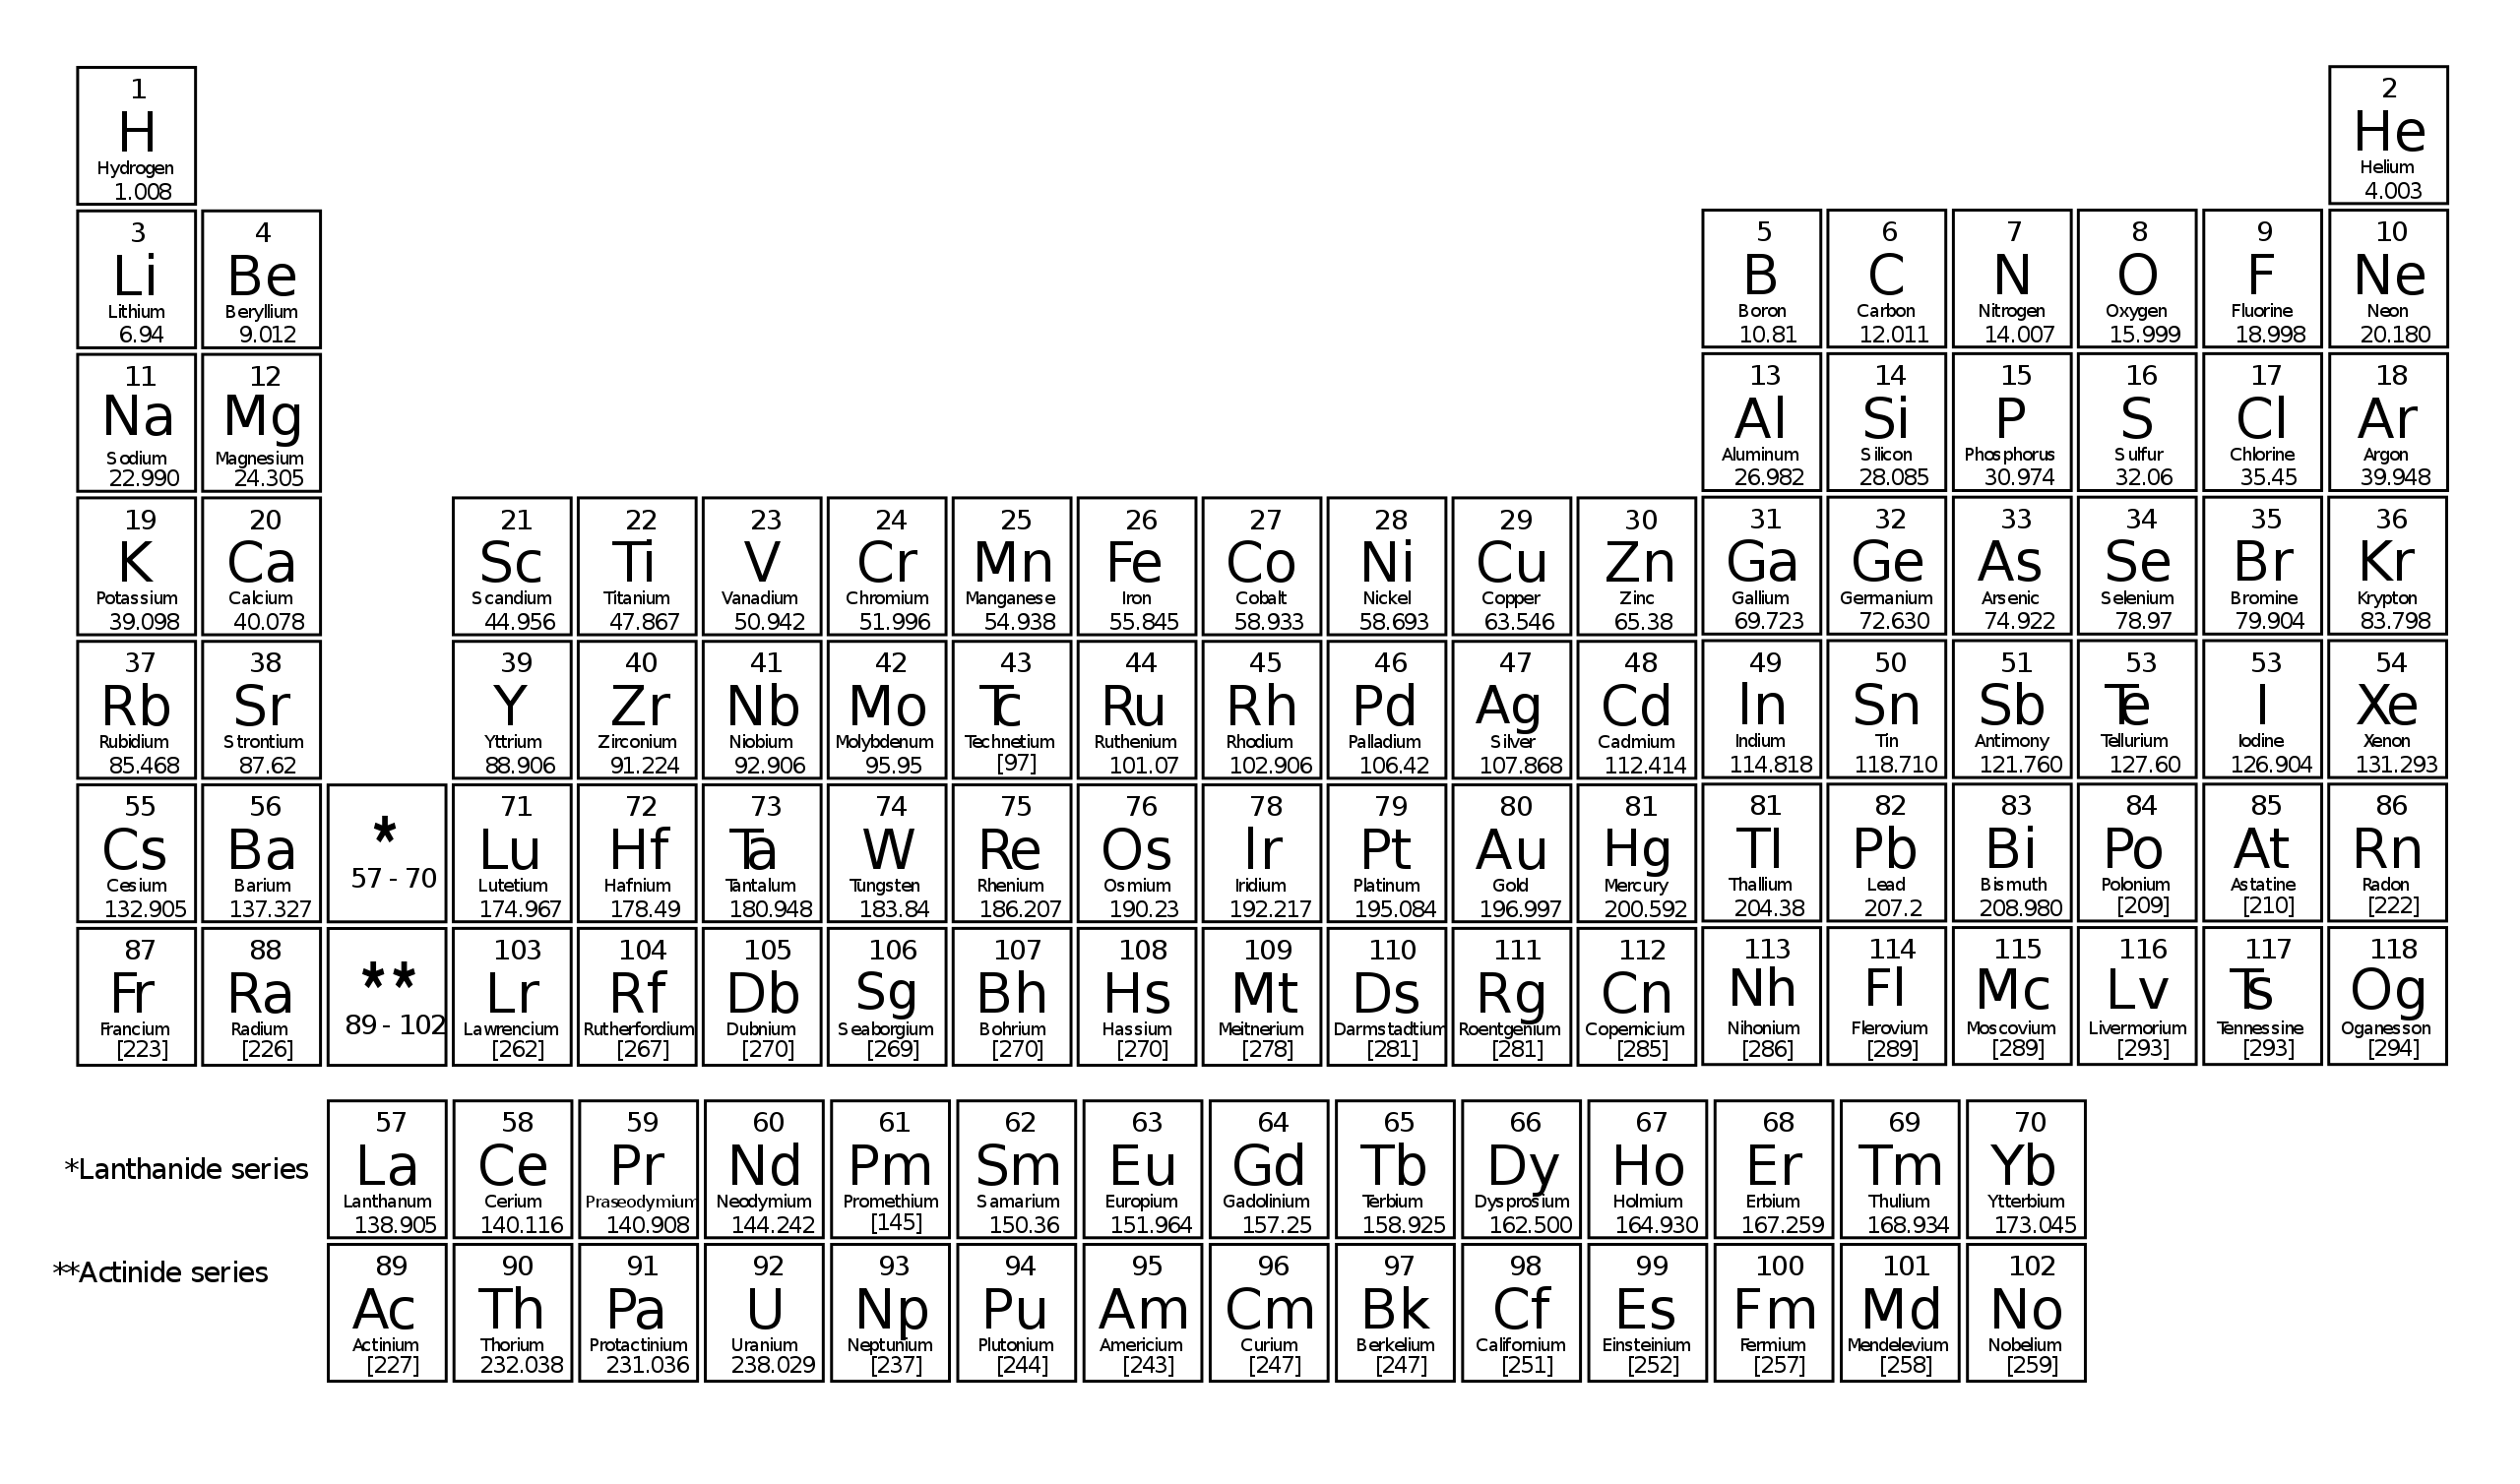
\includegraphics[scale=0.24,angle=90]{periodic_table}
\end{center}

\section{Apppendix 2 - Formulas and Constants}

\begin{align*}
  q = & mC\Delta T \\
  E = & \frac{hc}{\lambda} = h\nu \\
  h = & 6.626 \times 10^{-34} \text{J s} \\
  c = & \lambda \nu \\
  c = & 3.00 \times 10^8 \text{m/s}
\end{align*}
\end{document}
